
\chapter{Introduction}

This guide gives a first inside in how to write a standalone webservice for KnowArc including a suited client.
The practically oriented examples will be followed by explanations of the main architecture concepts.
For being able to comprehense basic knowledge of the programming language C++, the file format XML and the shell is requried.
Furthermore an installation of KnowArc 1 is needed.\\


The KnowArc server provides access to services which are used by clients. The services may cover computational tasks as well 
as access to a database. % job submission
Servers provide access to a certain service and are waiting for a client which demands it. The task of servers can be subdivided into:
\begin{itemize}
 \item Wait for client request
 \item Receive the request
 \item Perform the desired service
 \item Create a response for the client
 \item Send response to the client
 \item Wait for next client request
\end{itemize}
While the server waits passively for a request, the client acts actively:
\begin{itemize}
 \item Create a request
 \item Transmit the request to the server which provides the desired service.
 \item Receive the response from the server.
 \end{itemize}
\forcelinebreak

In general the implementation of a client is easier to be done compared with the server. 
KnowArc is designed as a middleware which encapsulates typical challenges of server-client infrastructures (security, exception handling, extensibility) and abstract from underlying architecture (heterogenous computer, computer location, protocols).
The core of KnowArc is the HED (Hosting Environment Daemon). HED is model consisting of a variable amount of heavily configurable layers. 
%
In the present case the endpoint of the HED will be a SOAP based Web Service. These Web Services exchange messages enveloped in the well known XML format. KnowArc abstracts from this format but nevertheless it is useful to be aware of the underlying message transport mechanism.\\
%which implicate several advantages.
%The XML file format is not restricted to a certain set of tags but can be expanded in such a way as to fit almost any kind of service. It is not a proprietary format and as a result many libraries in almost any language are capable in creating that kind of format.Likewise, XML is also suitable for the usage between heterogeneous platforms.However, while the client can be implemented very straight, the service has to fit a certain layout.In the present guide four kinds of webservices will be introduced: a simple time service, an echo service, a secure echo service and a service with a persistence state .\\


The source code of the examples given in this tutorial are available in the directory \textit{src}.
\task{All examples can be found in the source tree: URL}




\section{Hosting Environment Daemon}

The HED which was already mentioned in the section above is an essential part of the ARC middleware. It provides hosting of various services at application level, as well as a number of modules~\cite{QIANG_2005}. Figure~\ref{fig:HED_internal} illustrates a typical setup of a server sided HED. The HED consists of a few compononents called Message Chain Components (MCC) which are ordered within a layered structure and several \textcolor{urgent}{modules} which shall aid the programmer to simplify the development of the Web Services (Config, Loader, Logging, XMLNode).
%
\begin{figure}
	\centering
	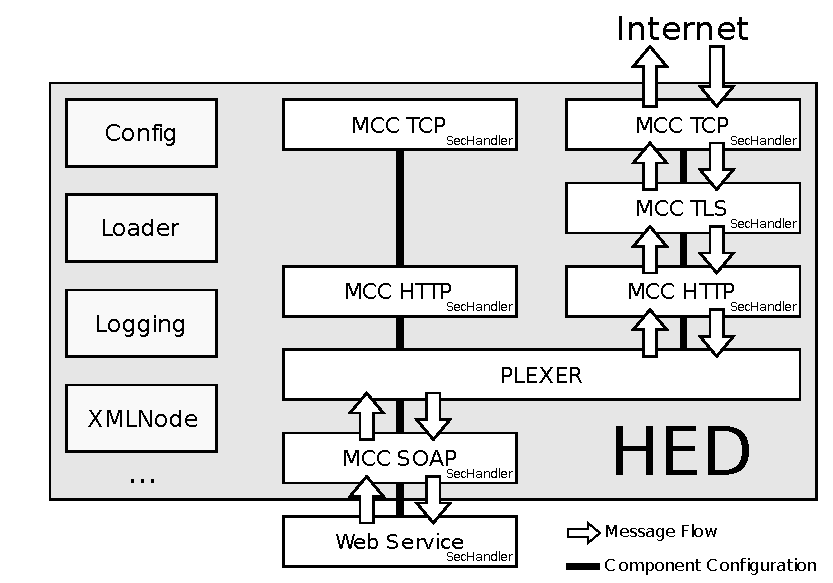
\includegraphics[width=14cm]{tex_introduction/HED.pdf}
	\mycaption{Example of HED structure with an Arex service and a file service.\task{ Replace image by an easier one!} }{\task{Write more stuff}\task{The images of the HED structure always are ordered like: TCP - TLS - HTTP - PLEXER - SOAP - WEB SERVICE   but the source code examples are: TCP - TLS - HTTP - SOAP - PLEXER - WEB SERVICE}}
\label{fig:HED_internal}
\end{figure}
The MCCs are passing the incoming and outgoing messages to the upper or the respective lower layer.
% AUFZÄHLUNG???
The lowest layer has to be a transport protocol like TCP which enables the transmission between the two applications, the client and the server. (The Internet Protocol (IP) beneath the TCP layer enables a transmission between two computers. IP is needed but not part of the HED.) TCP is well suited for the application because it provides a reliable and ordered delivery of a byte stream which is important to ensure security and a requirement for the usage of HTTP.
The TCP layer is followed by the Hypertext Transfer Protocol (HTTP). 
In case a security layer is desired, the TLS (Transport Layer Security formerly known as SSL, Secure Sockets Layer) can be inserted between the two layers TCP and HTTP.
The HTTP provides the client server architecture. It is stateless but offers several extensions for requests, header information and status codes. Furthermore HTTP enables the usage of Uniform Resource Locators (URL) which is used by KnowArc to multiplex between different services. The multiplexing layer needs to be defined within the HED and is called Plexer. Depending on the path of the URL the Plexer passes messages to a defined SOAP service which again passes the message to the Web Service.\\


The structure of the HED can be configured freely by modifying the HED configuration file. A first impression how the HED can be configured shall be given in the following example which corresponds to the HED shown in figure~\ref{fig:HED_internal}. It uses the internal ARC Echo service.



\subsection{The Arcecho service}
\task{Maybe the word tag needs to be replaced by the word element...}
\task{Where is the xsd file for HED configuration files??}
The first example shall give a basic understanding in how to configure the HED. The task is to setup the ARC intern Echo Web Service which has to be done by invoking the \textit{arched} daemon with a fitting HED configuration file. Such a fitting HED configuration file is shown in Listing~\ref{lst:arched_arcecho_xml}. It is written in XML and its structure is based on the \textcolor{urgent}{??} schema.
\lstsetARCHEDXML\\
\begin{program}
\centering
\lstinputlisting
	[
	label=lst:arched_arcecho_xml,
	caption={[HED configuration. Filename: arcecho\_no\_ssl.xml]
	\textbf{HED configuration. Filename: arcecho\_no\_ssl.xml\textcolor{white}{hmf}}}
	]
{../src/services/arched_arcecho.xml}
\end{program}
The first line of the XML file contains the XML declartion. Several attributes can be defined here but at least the XML version should be specified. \task{What is this ArcConfig for??} % configuration namespaces
The \textit{Server} tag, to be found at line~\ref{lst_code:arched_arcecho_Server}, provides basic settings for the daemon such as location of the Pid-file or the Log-file.
The \textit{ModuleManager} holds the path to the plugin libraries. Several paths may be defined here. Due to the fact that the first library fitting to the plugin name is loaded, the order is relevant. The path should be at least assigned to the ARC installation directory. % for the standard MCC are defined here
The next set of tags are holding the name of the plugins to be loaded (line~\ref{lst_code:arched_arcecho_Plugins}).
The names have to correspond to the name of the dynamic libraries within the path defined by the \textit{ModuleManager}.
Finally the chain of the components are declared initiate with the tag \textit{Chain}.
Each component inside the chain is represented by a tag called \textit{Component} which has at least a name attribute.
Its important that a plugin has been loaded which provides the functionality of it.
Depending on the component certain additional tags may be defined inside of it.
\task{Internet Protocol is required.}
The first component of the chain is the \textit{tcp.service}. As to be seen the port 60000 gets assigned for the server to listen to.
The stream which is received by this component is passed to the component defined by the \textit{next} tag.
In that case the will be passed to the component with the \textit{id} atrribute named \textit{http}. According to this manner the message will be passed to higher layers until it reaches the \textit{Plexer}  Depending on the path of the URL which was demanded by the HTTP the Plexer multiplexes the request to the right Web Service. The path is declared within the \textit{next} tag is a regular expression and leads to the service with the id named \textit{echo}. 
Which means that the service will be now reachable under URL \textit{http://localhost:60000/echo}.
This service finally will process the message and create a new message which will be returned all the way back to the TCP layer. The Echo Web Service itself is provided by the ARC package. Additional fix parameters can be passed by assigning tags which have to be known to the Web Service.
The tags \textit{echo:prefix} and \textit{echo:suffix} seen in this example are defining the characters which will enclose the echo  returned string.
\task{The images of the HED structure always are ordered like: TCP - TLS - HTTP - PLEXER - SOAP - WEB SERVICE   but the source code examples are: TCP - TLS - HTTP - SOAP - PLEXER - WEB SERVICE}\\


To create the daemon corresponding to the defined HED configuration file ARC-1 provides the program \textit{arched}.
The manner of invokation can been seen in Listing~\ref{lst:arcecho_arched_invokation}.
\lstsetKSH
\begin{program}
\begin{lstlisting}[
label=lst:arcecho_arched_invokation,
caption={[Invokation of the Arched Daemon.]
         \textbf{Invokation of the Arched Daemon.\textcolor{white}{hmf}}}]

$ arched -c arcecho_no_ssl.xml && echo Daemon started || echo Daemon start failed
 Daemon started
$
\end{lstlisting}
\end{program}
% $ rm -f /var/log/arched.log
% $ tail -n100 -f /var/log/arched.log
%...
%$ killall arched
%
%
The command is followed by the parameter \textit{c} which assignes, that the next string contains the full path of configuration file.
Once the server is running, the client can be used as described in Listing~\ref{lst:arcecho_client_invokation}.
\lstsetKSH
\begin{program}
\begin{lstlisting}[
label=lst:arcecho_client_invokation,
caption={[Usage of the Arc echo client.]
         \textbf{Usage of the Arc echo client.\textcolor{white}{hmf}}}]
$ arcecho http://localhost:60000/Echo text
[ text ]
\end{lstlisting}
\end{program}
In this example the server and the client are running on the same computer. For debugging it is advisable to check the Log-file which was assigned inside the HED configuration file.\\


In the following chapters own Web Services will be developed. Starting with the simple Time Web Service.












